The innate abilities that human beings possess to process complex things effortlessly in daily life are impressive. To translate even the fractional part of one of these abilities of the human being into a machine is a challenging task in itself. One such ability is to navigate in a social environment. For example, when we walk in a crowded public space we follow a large number of common-sense rules and social etiquette. Which includes respecting the personal space of others, yielding right-of-way, avoiding walking through the people belonging to the same group, taking the shortest path or safer path to the destination, and much more.

This ability of ours in the field of technology is known as Human/Pedestrian trajectory prediction. The task of predicting human trajectories is crucial for current and future technological advancements. Many end-user applications make intensive use of data analytics about pedestrians motion: urban safety, city planning, marketing, autonomous driving, to name a few. Typically, this implies the recollection and the offline analysis of these data, for understanding the pedestrian's behavior and taking decisions about the environment. In some contexts, however, one needs to go further and anticipate, in an online way, what will be the next pedestrian moves and infer their short or mid-term intentions. This allows to trigger early alarms or to take preventive actions when monitoring systems with critical real-time decision-making processes. In the case of autonomous driving, for example, inferring the intention of the pedestrians surrounding the car is of paramount importance in avoiding collisions. Many researchers have proposed miscellaneous approaches that tackle this problem. Helbing and Molnar~\cite{Helbing95} propose the Social Force model. Yi~\cite{Yi15} introduces the factor of a stationary group to the modeling of pedestrians trajectories with an energy map. The aforementioned ways are deterministic ways for prediction, they can not utilize the valuable information in the trajectories data.

\begin{figure}[h]
  \centering
  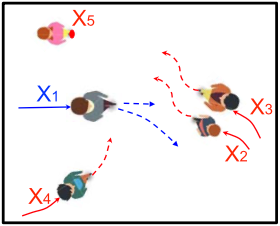
\includegraphics[width=\linewidth]{figures/fig-1.png}
  \caption{Pedestrian trajectory prediction is the task of predicting the future trajectories (dashed) of all humans which conform to the social norms, given the past observed scene (solid). The presence of social interactions distinguish human trajectory prediction from other sequence modelling tasks: the primary pedestrian (X1) deviates from his direction of motion to avoid a collision, by predicting the trajectory of the child (X2). \label{fig:fig-1}\protect\cite[]{HTF:DBLP:journals/corr/abs-2007-03639}}
  \Description{Figure extracted from "Human Trajectory Forecasting in Crowds: A Deep Learning Perspective"}
\end{figure}

Over the last few years, following the widespread usage of machine learning and deep learning methods, researchers use various neural networks to tackle the trajectories prediction problem. Zhou et al.~\cite{Zhou} build a linear dynamic system, applying Expectation Maximization (EM) algorithm to estimate parameters, to learn motion patterns in crowded scenes. Altché~\cite{Altche17} proposes a method that predicts the trajectory on the highway using Long Short-Term Memory (LSTM). Alahi et al.~\cite{Alahi16} give a sequence model based on LSTM as well as a social pooling that aggregates the human-human interaction in a scene.

However, these approaches mentioned previously learn only the pattern of human motion from data. Predicting human trajectory is a complex task. This is because both internal and external stimuli, such as intentions and other directly or indirectly observable influences, can affect human motion, as mentioned in the survey~\cite{humanmotionsurvey}. In addition to the location, which is usually recorded in the dataset, many factors that are not explicitly recorded in the dataset, such as speed, direction, or even not recorded, such as route and human intent. Recent researches have shown that Generative Adversarial Network (GAN) can better capture these uncertainties with latent space and thus naturally preserve multimodality. Gupta et al.~\cite{Gupta_2018_CVPR} used GAN and a Pooling Module to predict socially acceptable trajectories and found that certain directions in the latent space are related to direction and velocity. What is more, the study of Amirian et al.~\cite{Amirian_2019_CVPR_Workshops} has shown that InfoGAN, an information-theoretic extension to the Generative Adversarial Network~\cite{infogan}, partly improves the performance on commonly used datasets that have the largest variance in the prediction distribution, while still leaving some room for improvement.

Even though these researches give various effective models that fulfill the prediction task and attempt to encompass hidden aspects that influence the trajectory, they have not disentangled these factors in the latent space. If we know the factors that affect pedestrians' trajectory and apply these factors in specific scenarios, we can obtain better performance of prediction on various distributed datasets and to mitigate the limitations of the observed data. Therefore, we decide to consider the hidden factors behind different datasets.

In this study, we focus on what factors we can obtain that influence human trajectories and try to develop a model that can be controlled by these factors. we assume that different datasets have different static environments and so the data in a dataset share some specific common features. We consider three factors: obstacles (obstacles information such as the presence of static obstacles and the coordinates), maps (geometry and topology), and semantics (environment semantics such as no-go-zones, crosswalks, sidewalks, or traffic lights) in static environments, which are denoted by the survey~\cite{humanmotionsurvey}. We propose to develop a controllable generation model that is controlled by factor $c$ to have different static environments. We demonstrate that human movement is influenced by these three factors that we consider in a static environment. Also, with inputting different factors in static environments, our model can achieve better performance on different datasets.